\documentclass[12pt]{article}

\usepackage{times}
\usepackage{graphicx}
\usepackage{amsmath}
\usepackage{url}

\setlength{\textwidth}{6.5in}
\setlength{\textheight}{8.9in}
\setlength{\oddsidemargin}{0.0in}
\setlength{\topmargin}{0.05in}
\setlength{\headheight}{-0.05in}
\setlength{\headsep}{0.0in}

\newcommand{\indep}{\perp\!\!\!\perp}

\begin{document}

\begin{center}
{\bf CS 6300} \hfill {\large\bf HW08: Bayes Nets II \hfill {\bf Ryan Dalby} \hfill Due April 12, 2022}
\end{center}

\noindent
Please use the \LaTeX\ template to produce your writeups.  Hand in
using gradescope.

\section{Variable Elimination}

As an anthropologist, you are studying ancient human races.  You are
also a performing artist, and have an excellent model of the way
humans invent music and dance.  The key variables are:

\begin{description}

\item[Writing (W):] Whether or not a race invented some form of writing

\item[Cold climate (C):] Whether or not the race lived in a cold weather climate

\item[Music (M):] Whether or not a race invented music

\item[Tools (T):] Whether or not a race had metal tools

\end{description}

\noindent
You model the relationships between these variables and {\bf dance (D)}
using the Bayes net below.

\begin{center}
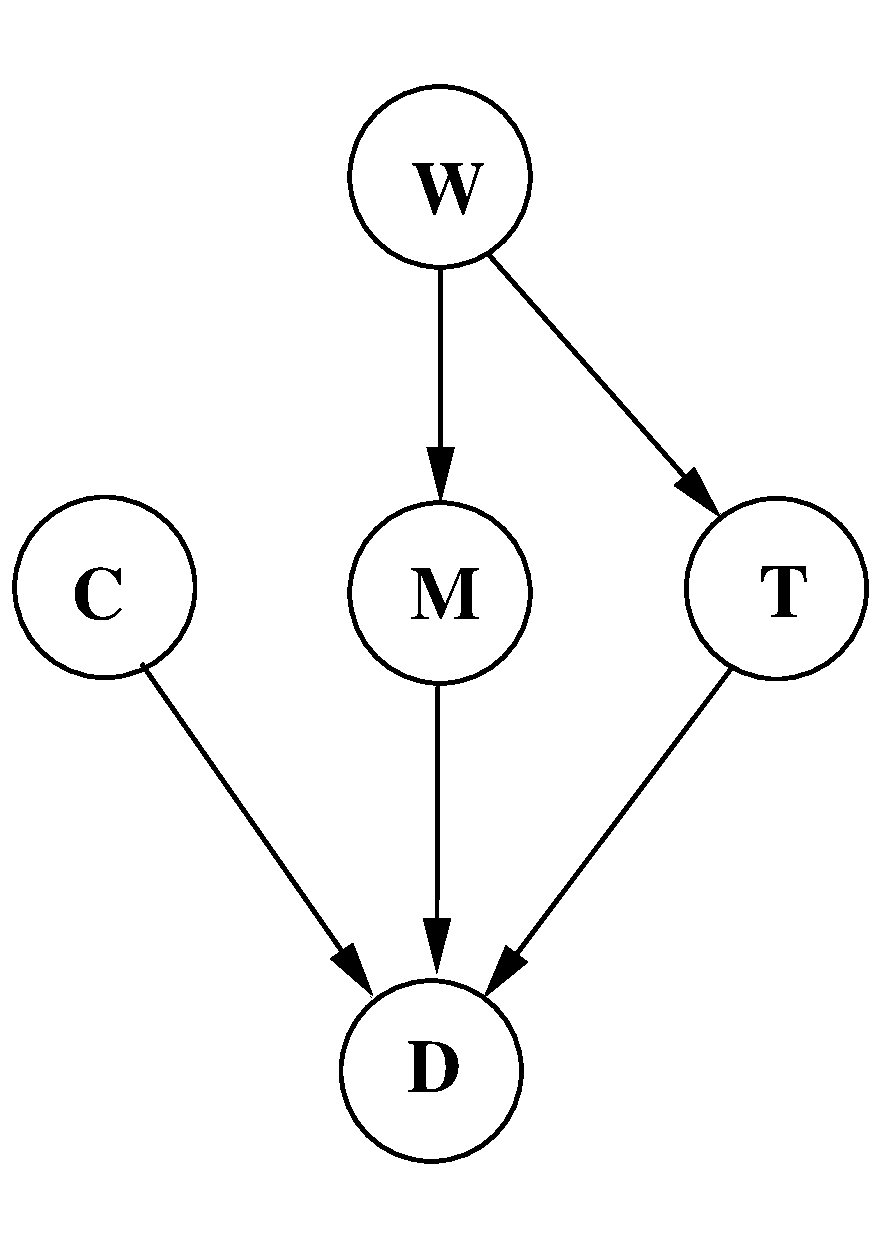
\includegraphics[height=3in]{dance1.eps}
\end{center}

\noindent
The conditional probabilities of the Bayes net are listed below.

$$\begin{array}{ccc}
\begin{array}{|c|c|c|c|c|} \hline
C  & M  & T  & D  & P(D|C,M,T) \\ \hline
+c & +m & +t & +d & 0.9 \\
+c & +m & +t & -d & 0.1 \\
+c & +m & -t & +d & 0.8 \\
+c & +m & -t & -d & 0.2 \\
+c & -m & +t & +d & 0.8 \\
+c & -m & +t & -d & 0.2 \\
+c & -m & -t & +d & 0.2 \\
+c & -m & -t & -d & 0.8 \\
-c & +m & +t & +d & 0.8 \\
-c & +m & +t & -d & 0.2 \\
-c & +m & -t & +d & 0.5 \\
-c & +m & -t & -d & 0.5 \\
-c & -m & +t & +d & 0.6 \\
-c & -m & +t & -d & 0.4 \\
-c & -m & -t & +d & 0.1 \\
-c & -m & -t & -d & 0.9 \\\hline
\end{array} &
\begin{array}{c}
\begin{array}{|c|c|c|} \hline
W  & M  & P(M|W) \\ \hline
+w & +m & 0.8 \\
+w & -m & 0.2 \\
-w & +m & 0.1 \\
-w & -m & 0.9 \\ \hline
\end{array} \\
 \\
\begin{array}{|c|c|c|} \hline
W  & T  & P(T|W) \\ \hline
+w & +t & 0.7 \\
+w & -t & 0.3 \\
-w & +t & 0.9 \\
-w & -t & 0.1 \\ \hline
\end{array}
\end{array} &
\begin{array}{c}
\begin{array}{|c|c|} \hline
W  & P(W) \\ \hline
+w & 0.9  \\
-w & 0.1  \\ \hline
\end{array} \\
 \\
\begin{array}{|c|c|} \hline
C  & P(C) \\ \hline
+c & 0.5  \\
-c & 0.5  \\ \hline
\end{array}
\end{array}
\end{array}$$

\noindent
You want to know how likely it is for a dancing, writing race to
invent music.

\begin{enumerate}

\item Write the formula to compute $P(+m | +d, +w)$ using variable elimination.

$P(M|+d,+w)$ will be found using variable elimination. 

Note $\times$ denotes pairwise multiplication.
Also note that not just $P(+m|+d,+w)$ was found since $P(M|+d,+w)$ must be known to compute the normalization factor $\alpha$.
\[
  P(M|+d,+w) = \alpha P(M,+d,+w) = \alpha \sum_C \sum_T P(C,M,T,+d,+w)
\]
\[
  P(M|+d,+w) = \alpha \sum_C \sum_T P(M|+w) P(T|+w) P(+d|C,M,T) P(+w) P(C)
\]
\[
  P(M|+d,+w) = \alpha P(+w) P(M|+w) \sum_C \sum_T P(T|+w) P(+d|C,M,T) P(C)
\]

In terms of initial factors
\[
  P(M|+d,+w) = \alpha f_1 \times f_2(M) \times \sum_C \sum_T f_3(T) \times f_4(C,M,T) \times f_5(C)
\]

where $f_1 = P(+w)$, $f_2(M) = P(M|+w)$, $f_3(T) = P(T|+w)$, $f_4(C,M,T) = P(+d|C,M,T)$, and $f_5(C) = P(C)$ 

Then joining and marginalizing factors as follows 
\[
  f_6(M) = \sum_C \sum_T f_3(T) \times f_4(C,M,T) \times f_5(C)
\]
\begin{gather}
  f_6(M) = f_3(+t) f_4(+c,M,+t) f_5(+c) + f_3(-t) f_4(+c,M,-t) f_5(+c) + \\
  f_3(+t) f_4(-c,M,+t) f_5(-c) + f_3(-t) f_4(-c,M,-t) f_5(-c)
\end{gather}
\[
  f_7(M) = f_2(M) \times f_6(M)
\]
\[
  f_8(M) = f_1 \times f_7(M)
\]

Gives
\[
  P(M|+d,+w) = \alpha f_8(M)
\]


\item Now compute $P(+m | +d, +w)$.

\[
  f_1 = 0.9
\]

\begin{center}
  \begin{tabular}{|c|c|}
    \hline
    $M$ & $f_2(M)$ \\
    \hline
    $+m$ & 0.8 \\
    \hline
    $-m$ & 0.2 \\
    \hline
  \end{tabular}

  \begin{tabular}{|c|c|}
    \hline
    $T$ & $f_3(T)$ \\
    \hline
    $+t$ & 0.7 \\
    \hline
    $-t$ & 0.3 \\
    \hline
  \end{tabular}

  \begin{tabular}{|c|c|c|c|}
    \hline
    $C$ & $M$ & $T$ & $f_4(C,M,T)$ \\
    \hline
    $+c$ & $+m$ & $+t$ & 0.9 \\
    \hline
    $+c$ & $+m$ & $-t$ & 0.8 \\
    \hline
    $+c$ & $-m$ & $+t$ & 0.8 \\
    \hline
    $+c$ & $-m$ & $-t$ & 0.2 \\
    \hline
    $-c$ & $+m$ & $+t$ & 0.8 \\
    \hline
    $-c$ & $+m$ & $-t$ & 0.5 \\
    \hline
    $-c$ & $-m$ & $+t$ & 0.6 \\
    \hline
    $-c$ & $-m$ & $-t$ & 0.1 \\
    \hline
  \end{tabular}

  \begin{tabular}{|c|c|}
    \hline
    $C$ & $f_5(M)$ \\
    \hline
    $+c$ & 0.5 \\
    \hline
    $-c$ & 0.5 \\
    \hline
  \end{tabular}

  \begin{tabular}{|c|c|}
    \hline
    $M$ & $f_6(M)$ \\
    \hline
    $+m$ & 0.79 \\
    \hline
    $-m$ & 0.535 \\
    \hline
  \end{tabular}

  \begin{tabular}{|c|c|}
    \hline
    $M$ & $f_7(M)$ \\
    \hline
    $+m$ & 0.632 \\
    \hline
    $-m$ & 0.107 \\
    \hline
  \end{tabular}

  \begin{tabular}{|c|c|}
    \hline
    $M$ & $f_8(M)$ \\
    \hline
    $+m$ & 0.5688 \\
    \hline
    $-m$ & 0.0963 \\
    \hline
  \end{tabular}

  Normalizing by $\alpha = 1.5035$

  \begin{tabular}{|c|c|}
    \hline
    $M$ & $P(M|+d,+w)$ \\
    \hline
    $+m$ & 0.855 \\
    \hline
    $-m$ & 0.145 \\
    \hline
  \end{tabular}
\end{center}

Thus $P(+m|+d,+w) = 0.855$.

\end{enumerate}

\clearpage

\section{Sampling}

You decide to use sampling instead.  You use prior sampling to draw
the samples below:

$$\begin{array}{|c|c|c|c|c|} \hline
W  & C  & M  & T  & D  \\ \hline
-w & +c & +m & -t & +d \\
+w & +c & -m & -t & -d \\
+w & -c & -m & +t & -d \\
+w & +c & +m & -t & +d \\
+w & +c & -m & +t & +d \\
+w & -c & -m & +t & -d \\
+w & -c & -m & -t & -d \\
+w & +c & +m & +t & +d \\
+w & +c & -m & +t & -d \\
-w & -c & -m & -t & -d \\ \hline
\end{array}$$

\begin{enumerate}

\item Based on rejection sampling using the samples above, what is the
  answer to your query $P(+m | +d, +w)$?

Given that we have sampled already, we just reject/ignore all samples without $D=+d$ and $W=+w$.

Looking at the remaining samples: 
$$\begin{array}{|c|c|c|c|c|} \hline
W  & C  & M  & T  & D  \\ \hline
+w & +c & +m & -t & +d \\
+w & +c & -m & +t & +d \\
+w & +c & +m & +t & +d \\ \hline
\end{array}$$

We have 2 counts of $+m$ and 1 count of $-m$ thus we normalize by $\alpha = \frac{1}{3}$. 
We get our estimate of $P(+m|+d,+w) = \frac{2}{3} \approx 0.667$.

\item While your sampling method has worked fairly well in many cases,
  for rare cases (like a race that doesn't write) your results
  are less accurate as rejection sampling rejects almost all of the
  data.  You decide to use likelihood weighting instead.

You now wish to compute the probability that a race that has no
writing ($-w$) or dancing ($-d$) nonetheless has music ($+m$), using
likelihood weighting. I.e., you want $P(+m | -w, -d)$.

\begin{enumerate}

\item You draw four samples, using likelihood weighting.  The
  following random numbers are generated, used in the order CT.

\begin{center}
0.45 0.85 0.12 0.95 0.66 0.23 0.07 0.46 
\end{center}

Complete the following tables with the four samples.

$$\begin{array}{|c|c|c|c|c|c|} \hline
W  & C  & M  & T  & D  & \hbox{weight} \\ \hline
-w & +c & +m & +t & -d & (0.1)(0.1)=0.01\\
-w & +c & -m & -t & -d & (0.1)(0.8)=0.08\\
-w & -c & -m & +t & -d & (0.1)(0.4)=0.04\\
-w & +c & +m & +t & -d & (0.1)(0.1)=0.01\\ \hline
\end{array}$$

\item For each of these samples, indicate its weight in the same table.

See the table.

\item Compute the answer to your query, $P(+m | -w, -d)$, using
  likelihood weighting with these samples.

\[
  P(+m|-w,-d) = \frac{0.01+0.01}{0.01+0.08+0.04+0.01} = 0.143
\]

\end{enumerate}

\end{enumerate}

\end{document}


